\documentclass[12pt]{exam}
\usepackage[utf8]{inputenc}

\usepackage[margin=1in]{geometry}
\usepackage{amsmath,amssymb}
\usepackage{multicol}
\usepackage{hyperref}
\usepackage{graphicx}
\usepackage{color}


\newcommand{\class}{CS 5060}
\newcommand{\term}{Fall 2024}
\newcommand{\examnum}{Midterm Exam}
\newcommand{\examdate}{10/10/2024}
\newcommand{\timelimit}{10/14/2024 By End of Day}


\pagestyle{head}
\firstpageheader{}{}{}
\runningheader{\class}{\examnum\ - Page \thepage\ of \numpages}{\examdate}
\runningheadrule


\begin{document}

\noindent
\begin{tabular*}{\textwidth}{l @{\extracolsep{\fill}} r @{\extracolsep{6pt}} l}
\textbf{\class} & \textbf{Name:} & \makebox[2in]{\hrulefill}\\
\textbf{\term} &&\\
\textbf{\examnum} &&\\
\textbf{\examdate} &&\\
\textbf{Time Limit: \timelimit} & \makebox[2in]{\hrulefill}
\end{tabular*}\\
\rule[2ex]{\textwidth}{2pt}

This exam contains \numpages\ pages (including this cover page) and \numquestions\ questions.\\
The total of points is \numpoints.

This test is open notes but not open-neighbor.  Please read each question carefully before deciding on an answer.  A clear and concise statement or paragraph is much better than long answers with no focus on short written responses to these questions. 

I have taken the liberty of organizing this as I would an assignment rather than a classical exam. I hope that you take the time to learn and understand this. I imagine this will be a moderately pleasant venture if you do so.

Mario Mercy Option: As long as you get 3 of these questions with 75\%, the overall exam score will be at least 75\%.



\begin{center}
Grade Table \\
\addpoints
\gradetable[v][questions]
\end{center}

\noindent
\rule[2ex]{\textwidth}{2pt}

\begin{questions}


\question[20] Question 1: Algorithm Pseudocode (40 points)
\addpoints

Write pseudocode to describe the following four algorithms:

\begin{itemize}
    \item \textbf{Optimal Stopping Problem}: Describe the process of stopping optimally to maximize the expected reward.
    \item \textbf{Multi-Armed Bandit Problem}: Write pseudocode for exploring and exploiting multiple options to maximize cumulative reward.
    \item \textbf{Option Valuation}: Provide pseudocode for calculating the value of a financial option, considering potential future prices.
    \item \textbf{Insurance Algorithm}: Detail the pseudocode for pricing an insurance product based on probabilistic risk models.
\end{itemize}

\textit{Each pseudocode description should include input, output, and a high-level explanation of key steps.}



\question[40] Question 2: Impact of Randomness on Algorithms (30 points)

Consider how randomness affects each of the algorithms discussed in Question 1. For each algorithm, explain how the behavior changes when using different random distributions (uniform, normal, and beta with skew).

\begin{itemize}
    \item How would the \textbf{Optimal Stop} algorithm change with these distributions?
    \item How does the \textbf{Multi-Armed Bandit} algorithm's decision-making change?
    \item How does the randomness impact the \textbf{Option Valuation} algorithm?
    \item How would randomness alter the performance of the \textbf{Insurance Algorithm}?
\end{itemize}

Additionally, consider the following example of an interesting distribution (shown in Figure \ref{fig:distribution}), and describe how you think it might impact these algorithms. Draw any connections between the shape of the distribution and potential algorithm behavior.


\begin{figure}
    \centering
    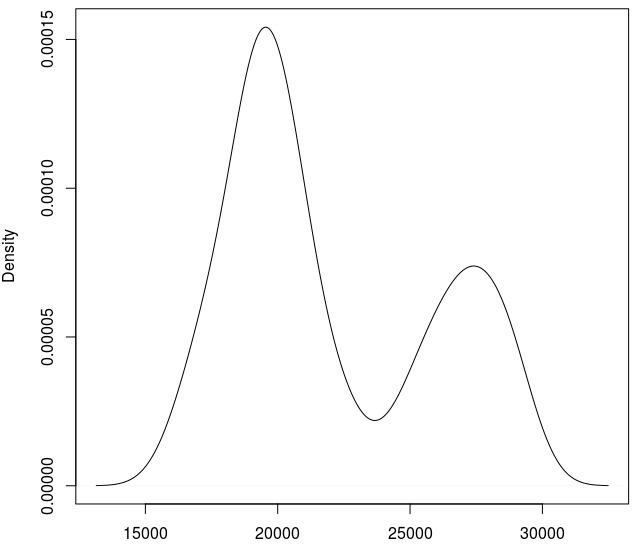
\includegraphics[width=0.75\linewidth]{interesting_distribution.png}
    \caption{A distribution that is fairly common in a certain type of field we have discussed at some length in our course lectures.}
    \label{fig:distribution}
\end{figure}


\question[20] Question 3: Nature of the Algorithms (20 points)

Discuss the following properties of the algorithms:

\begin{enumerate}
    \item \textbf{Topology in the Optimal Stop Algorithm}: How does the state-space or topology of decisions evolve? How does this affect finding the optimal stopping point?
    \item \textbf{Explore/Exploit Trade-offs in Multi-Armed Bandits}: How do different strategies (epsilon-greedy, Thompson sampling) handle the explore/exploit trade-off in various conditions?
    \item \textbf{Option Valuation Model}: How do assumptions (e.g., volatility, time) change the option valuation model? What might happen under extreme assumptions?
    \item \textbf{Effective Insurance Product Design}: What considerations improve the design of an insurance product? How does uncertainty and risk modeling influence pricing?
\end{enumerate}







% \question[20] Processor Binning:  
% \addpoints

% You are tasked with fulfilling a procurement request for a mission-critical component, the processor that your company makes is typically binned into three categories: Class 7, Class 5, and Class 3. (Side note: it is interesting that both team AMD and team Intel uses the same numerical designations...)

% Processors that passes the highest levels are given the 7 designation, with those that pass mid levels are given 5, and those that are very unstable have cores turned off and given the 3 designation. Our technique is very good, and we can have a success rate of 58\% viable processors. Of these processors, 67\% are Class 3, 24\% are Class 5, 8.8\% are Class 7, and 0.2\% are Extreme High Performance (EHP). 

% PART 1 - Set up the simulation with a random float drawn between 1-1000 to emulate the value of the processor. (Note that we must deliver one processor within one week to our client, but they can only accept our EHP products.) Run a simulation assuming we can fabricate and bin-test 1000 units per day. Plot the daily distribution of simulated EHP processors of at least 50 days.

% PART 2 - Compute the simple early stopping rule for this problem. Show some plots of the performance.

% PART 3 - Compute the stopping rule where we get a reward based on the following function:

% \begin{center}
%     $ 0$ if $val < 998 $ \\
%     $ 5000 * (val - 997)**2 $ if $ val >= 998 $
    
% \end{center}

% Again, show some plots of performance.

% PART 4 - We invest in a slower but better lithography method, increasing our base success rate to 69\%. In addition 48\% are now Class 3, 33\% are Class 5, and 14\% are class 5. The remaining 5\% are EHPs. Calculate the new results for the reward function in PART 3.

% How does this compare with the first simple early-stopping problem?



% \question[20] Mineral Samples and Geologic Surveys:
% \addpoints

% You are part of the algorithms team behind a large mining group, based on several survey team results, you have identified 10 potentially valuable locations to start mineral excavation. This is a very expensive process, and developed infrastructure capital is often not movable once installed. You are interested in conducting some pilot mining using inefficient, but cheaper (lots of small trucks) methods for a few months.

% The distribution of mineral value in each area looks as follows:

% area1 = beta(2, 2)+1\\
% area2 = beta(3, 7)*3\\
% area3 = normal(2.4, 1.8)\\
% area4 = uniform(-1, 4)\\
% area5 = normal(0, 9)\\
% area6 = beta(7, 3)+2\\
% area7 = uniform(0, 4)\\
% area8 = beta(3, 7)*2\\
% area9 = normal(2, 1.4)\\
% area10 = normal(1.3, 7)\\


% PART 1 - You have enough teams of trucks to collect data from each location simultaneously. Plot the results of conducting an equal test with one data point collected each month after your 2-year pilot study is completed. 

% PART 2 - You can remove resources to dedicate them to another operational site to get more data points per month. Each data point you get will be different as each team will start excavation in a different sub-area. You have funding for a 2-year pilot study, compute an epsilon greedy approach where each of your 10 teams can move. \color{red} Tell me what your logic is to move these teams and when \color{black}

% PART 3 - Lock the teams to be unable to move for 6 months. Allow each team to move in an epsilon-greedy fashion. How does your algorithm perform? show plots and comment on your changes.

% PART 4 - By the end of the 2-year pilot, operational funds are allocated to open an operational mine in two locations. Which did you pick, and how quickly were you able to determine what locations were best?




% \question[20] Tech Sector before the Covid changes:
% \addpoints

% Suppose that you are a bank that services many firms tied closely to the technology sector. We will be looking at specifically AAPL (Apple) and TSLA (Tesla) shares provided in the Canvas midterm module. 

% PART 1 - Plot the value of the assets over time, use the Close price column. Also, plot a distribution of the difference between the high and low prices each day. Plot the distribution of the change in prices of the close each day. Comment on the similarities and differences in these stocks. Explain the distributions which govern the change in Close price of these two stocks. 

% [10] PART 2 - Compute a 1-year European Call option moving forward from the final date in the data provided (Jan 31, 2020). The strike price is the same as the close price on that day. Assume volatility at 8.2\%. Calculate the drift based on a regression or analysis in PART 1. Use the distribution of the stocks calculated. Plot the simulated paths for 1000 runs and the computed answer.

% PART 3 - Find the option price for a new financial asset called the AAPL+TESLA security. This security is the value of the average between the two options. 

% Now add a simulated slide down in March of 2020 of 35\% for AAPL and 41\% for TSLA. What Happens to the price of the option if you could predict this slide in price from COVID?
% % \begin{figure}
% %     \centering
% %     \includegraphics[width=0.25\linewidth] {AAPL2020Covid.png}
% %     \caption{Enter Caption}
% %     \label{fig:enter-label}
% % \end{figure}
% (Assume the same 1-year window of expiry)

% PART 4 - BONUS QUESTION: Do PART 3 again but Calculate the joint probabilities through a correlation matrix and simulate random draws that reflect the correlation in these tech-heavy industries. Add the expected mid-COVID growth to the stock prices starting in April of 2020, where firms grew 3x faster than anticipated after a 30\% slump. 

\question[40] Insurance: Value of Subdivision
\addpoints

We are going to look at a simple insurance dataset (in the Canvas midterm module, a data file is provided named insurance.csv) where we only consider a few factors for 10,000 people: 

\begin{itemize}
    \item age (INT age of claimant)
    \item sex (BINARY As identified by the claimant)
    \item bmi (FLOAT bmi of claimant, NA if not claimant that year)
    \item children (INT children count per claimant, NA if not claimant that year)
    \item smoker (BINARY smoking status of claimant, NA if not claimant that year)
    \item region (STRING claimant regional ID, NA if not claimant that year)
\end{itemize}

PART 1 - Calculate the basic insurance rate for this population if we are looking at zero deductible policies and we need an 11 \% profit margin. What is the standard deviation and volatility of this portfolio?

PART 2 - Calculate the tiered insurance rate (with the same 11\% profit margin) for this population by breaking up the insurance product by age categories of [18-22, 23-30, 31-48, and 49+]. What is the standard deviation and volatility of this portfolio?

PART 3 - Calculate the same in PART 2, but add sex to the calculation. Compare just using the sex parameter as compared to both age and sex. 

PART 4 - Comment on the change in risk for the portfolio and the anticipated benefits from subdividing the insurance product. Calculate what the prices would be if you could break the product into known claimants (ie: you know which people will be claimants and who will not be this year). What does the cost rise to for the annual rate on the claimants? 





% \vspace{10mm}
% \noaddpoints
% Bonus: \question[3] I could really use help in understanding how to improve the course, particularly as I missed a few days. Thank you for being here and working hard on these topics. 

% What is making sense, and what doesn't? How can I do this better? (I know I can certainly post lectures faster... and clarify assignments better...)

\end{questions}


\end{document}
